\documentclass[11pt, oneside]{article} 
\usepackage{geometry}
\geometry{letterpaper} 
\usepackage{graphicx}
	
\usepackage{amssymb}
\usepackage{amsmath}
\usepackage{parskip}
\usepackage{color}
\usepackage{hyperref}

\graphicspath{{/Users/telliott_admin/Tex/png/}}
% \begin{center} 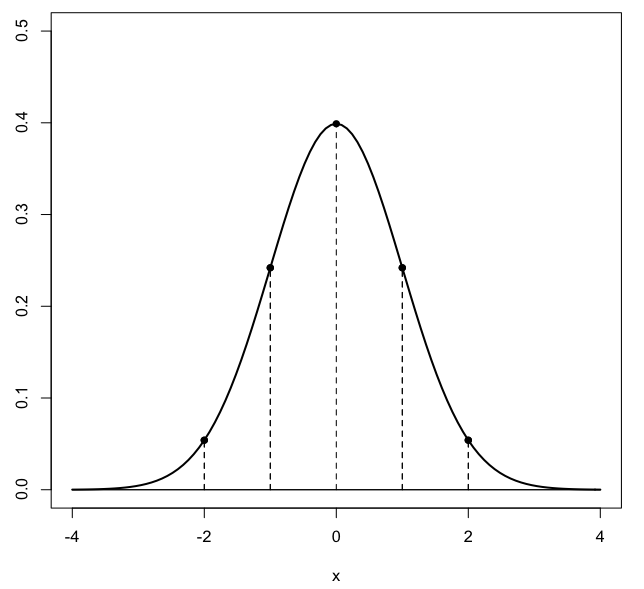
\includegraphics [scale=0.4] {gauss3.png} \end{center}

\title{Polar - summary}
\date{}

\begin{document}
\maketitle
\Large
\subsection*{circle}
A very simple circle in polar coordinates is $r = a$.  There is no $\theta$-dependence when the circle has its center at the origin.

For a circle of radius $a$ centered at $(a,0)$ then
\begin{center} 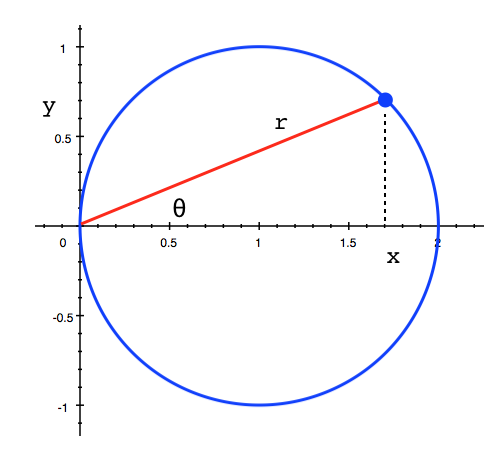
\includegraphics [scale=0.4] {polar_circle2.png} \end{center}
\[ a^2 = (x - a)^2 + y^2 \]
\[ x^2 - 2ax + y^2 = 0 \]
Always, $x = r \cos \theta$ and $y = r \sin \theta$ so
\[ r^2 (\sin^2 \theta + \cos^2 \theta)  - 2a r \cos \theta = 0 \]
\[ r^2  - 2a r \cos \theta = 0 \]
\[ r = 2a \cos \theta \]
If the center of the circle is on the $y$-axis the equation is similar but with $\sin \theta$.  A more general equation is
\[ r = 2h \cos \theta + 2k \sin \theta \]
which is a circle that touches the origin, and has its center at $(h,k)$.  

The most general equation is with the circle anywhere in the plane.  If we remember to specify the center at $(s, \phi)$ in \emph{radial} coordinates, then the law of cosines easily yields
\[ r^2 + s^2 - 2rs \cos (\theta - \phi) = a^2 \]

\subsection*{reverse}
Start from
\[ r = 2h \cos \theta + 2k \sin \theta \]
Always, $x = r \cos \theta$ and $y = r \sin \theta$ so
\[ r = 2h \frac{x}{r} + 2k \frac{y}{r} \]
\[ r^2 = 2hx + 2ky \]
\[ x^2 + y^2 = 2hx + 2ky \]
Easily rearrange and complete the square:
\[ x^2 - 2hx + h^2 + y^2 - 2ky + k^2 = h^2 + k^2 \]
\[ (x - h)^2 + (y - k)^2 =  h^2 + k^2 \]
For a circle touching the origin, $h^2 + k^2 = a^2$
\[ (x - h)^2 + (y - k)^2 =  a^2 \]

\subsection*{parabola}
To derive the equation for a parabola in polar coordinates it is convenient to rotate from the standard orientation by 90 degrees CW.  In this way $\theta$ will have its usual relationship with the $x$-axis.
\begin{center} 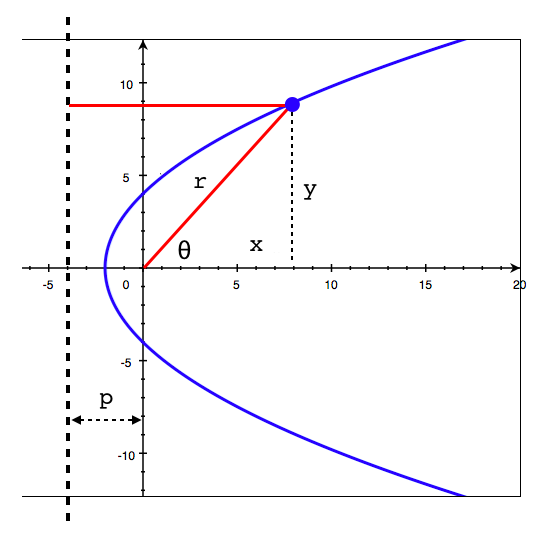
\includegraphics [scale=0.4] {polar_parabola.png} \end{center}
The origin of coordinates is placed at the focus, the distance to the vertex for this parabola is $2$, and the distance from the origin to the directrix is $p = 4$.
 
Note that in Cartesian coordinates, this parabola will be of the form is $x = ay^2$ because of the rotation.

The distance from the focus to a general point $(x,y)$ is just $r$.  The distance from the directrix to the point is $p + x$.  The geometric constraint gives simply:
\[ r = p + x \]
We make the standard substitution $x = r \cos \theta$.
\[ r = p + r \cos \theta \]
Some rearrangement gives the standard equation
\[ r = \frac{p}{1 - \cos \theta} \]
For a vertically oriented parabola we would have $\sin \theta$ instead.

\subsection*{reverse}
To go back to Cartesian coordinates, reverse the substitution for $x$:
\[ r = \frac{p}{1 - x/r} \]
\[ r - x = p \]
\[ r^2 = (x + p)^2 \]
Use $r^2 = x^2 + y^2$:
\[ x^2 + y^2 = x^2 + 2px + p^2 \]
\[ y^2 = 2px + p^2 \]
\[ \frac{1}{2p} y^2 = x + \frac{p}{2} \]

This looks unusual.  However, the equation that was actually plotted was $r = 4/(1 + \cos \theta)$ ($p = 4$).  

Note:  here we have used $p$ as the distance from the focus to the directrix, which is twice the distance to the vertex.  If we call the latter distance $c$, the $p = 2c$.  Previously we showed that $4ac = 1$, so $a = 1/4c$.  Thus we obtain $a = 1/8$:
\[ \frac{1}{8} y^2 = x + 2 \]
This shape factor matches the plot (four units above the axis (at $x=0$ is two units to the right of the vertex) and the vertex is at $(-2,0)$.  $a$ is unusually small, the reason is so the parabola will open quickly, giving room to put all the labels in the diagram.

\subsection*{ellipse}
From the geometry of the ellipse, with the center at the origin, it is fairly easy to show that
\[ a^2  = b^2 + c^2 \]
and derive the equation of the ellipse in Cartesian coordinates:
\[ \frac{x^2}{a^2} + \frac{y^2}{b^2} = 1 \]

To derive the equation for an ellipse in polar coordinates it is convenient to shift the origin of coordinates to be the left focus of the ellipse at $(-c,0)$.

\begin{center} 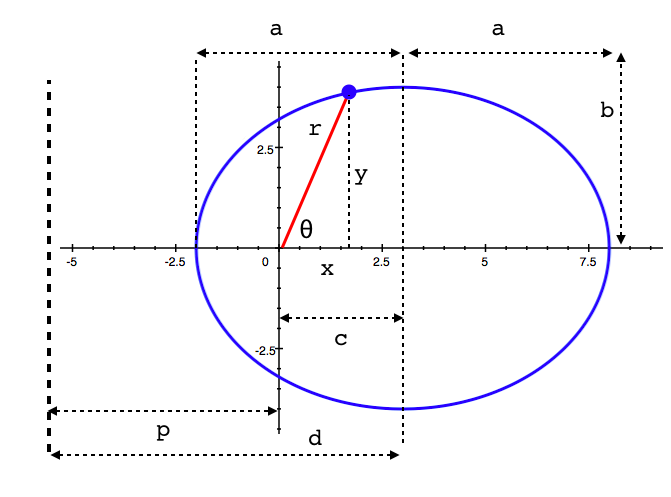
\includegraphics [scale=0.4] {polar_ellipse.png} \end{center}
The ellipse plotted here has $a = 5, b = 4$ and so $c = \sqrt{a^2 - b^2} = 3$.  It has been shifted so the focus at $(-3,0)$ is the origin of coordinates.

The eccentricity $e$ is defined by the geometric constraint (next), which can be shown to be equivalent to $c/a = 0.6$.  

Let $p$ be the distance from the focus to the directrix, and let $d$ be the distance from the directrix to the center of the ellipse.

The ellipse can be defined by its \textbf{geometric constraint}.

This says that for any point on the ellipse, the ratio of the distance from the focus (and here, the origin) to the point (that is, $r$), when divided by the distance from the point to the directrix, $x + p$, is equal to a constant, which we will call the eccentricity $e$.
\[ \frac{r}{x + p} = \frac{r}{p + r \cos \theta} = e \]
\[ r = e(p + r \cos \theta) \]

We simply rearrange to isolate $r$
\[ r(1 - e \cos \theta) = ep \]
\[ r = \frac{ep}{1 - e \cos \theta} \]

\subsection*{reverse}
Going back is more complicated for the ellipse. Reverse the substitution $x/r = \cos \theta$.
\[ r(1 - e x/r) = ep \]
\[ r - ex = ep \]
\[ r = ex + ep \]
There's a \emph{magic} substitution that we will justify below: 
\[ ep = a(1 - e^2) \]
Using that, we have
\[ r = ex + a(1-e^2) \]
Use $r^2 = x^2 + y^2$:
\[ x^2 + y^2 = e^2 x^2 + 2exa(1-e^2) + a^2(1- e^2)^2 \]
Combine cofactors for $x^2$, obtaining $(1-e^2)$ and then divide through by $(1-e^2)$: 
\[ x^2 + \frac{y^2}{1-e^2} = 2exa + a^2(1- e^2) \]
Complete the square for $x$ by adding $(ea)^2$ to both sides
\[ x^2 - 2exa + (ea)^2 + \frac{y^2}{1-e^2} = a^2(1- e^2) + (ea)^2 \]
\[ (x - ea)^2 + \frac{y^2}{1-e^2} = a^2(1- e^2) + (ea)^2 \]

We asserted that $ea = c$.  Simplify the right-hand side at the same time:
\[ (x - c)^2 + \frac{y^2}{1-e^2} = a^2 \]
This is great, because we need to shift the origin of coordinates back to the center of the ellipse by exactly this amount.

Unfortunately, I have not discovered any way to make that derivation simpler.  
\subsection*{solve for $1 - e^2$}

To deal with $1 - e^2$, recall that the basic geometry says
\[ a^2 - c^2 = b^2 \]
\[ 1 - (\frac{c}{a})^2 = \frac{b^2}{a^2} \]
Since $c = ea$
\[ 1 - e^2 = \frac{b^2}{a^2}  \]
so what we had simplifies as the inverse of that times $y^2$
\[ (x - c)^2 + \frac{a^2}{b^2} \ y^2 = a^2 \]
\[ \frac{(x - c)^2}{a^2} + \frac{y^2}{b^2} = 1 \]
Exactly what we want.  Furthermore, we can view this derivation in reverse as a proof of $c = ea$ for an ellipse with this equation in Cartesian coordinates, shifted out to focus $(-c,0)$.

Now let's explain the substitution:
\[ ep = a(1 - e^2) \]
It is easiest to start by finding an expression for $d$, then getting $e$ and $p$.
\begin{center} 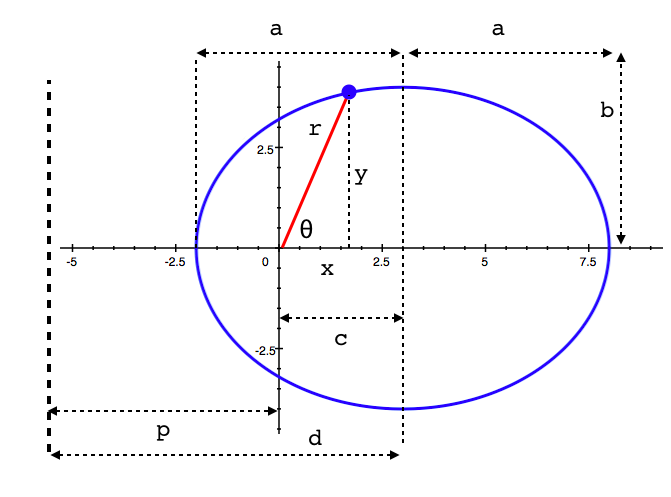
\includegraphics [scale=0.4] {polar_ellipse.png} \end{center}

\subsection*{solve for $d$ and $e$}
Applying the geometric constraint to the extreme left end:
\[ \frac{a - c}{d - a} = e  \]
At the very top of the ellipse the distance to the focus is $\sqrt{b^2 + c^2}$ but this is also just $a$, which means
\[ \frac{a}{d} = e = \frac{a - c}{d - a} \]
so 
\[ ad - a^2 = ad - cd \]
thus
\[ d = \frac{a^2}{c} \]
One can also obtain this result by equating the ratios for the left and right ends of the ellipse.  

Notice that the ratio $a/d$ obeys the geometric constraint:
\[ \frac{a}{d} = e = \frac{ac}{a^2} = \frac{c}{a} \]
We have proved $ae = c$, using only the geometry.

A longer, but pretty, proof is to start from the ratio for the extreme right end:
\[ e = \frac{a + c}{d + a} \]
substitute $d = a^2/c$
\[ = \frac{a + c}{a^2/c + a} \]
Multiply top and bottom by $1/a$
\[ e = \frac{1 + c/a}{a/c + 1} \]
Put top and bottom over common denominators
\[ e = \frac{(a + c)/a}{(a + c)/c} = \frac{c}{a} \]

\subsection*{solve for $p$}
\[ p = d - c = \frac{a^2}{c} - c \]
\[ = \frac{a^2 - c^2}{c} = \frac{b^2}{c} \]

\subsection*{finally}
\[ pe = \frac{b^2}{c} \cdot \frac{c}{a} = \frac{b^2}{a} \]
\[ = \frac{a^2 - c^2}{a} \]
\[ = \frac{a^2 - e^2a^2}{a} \]
\[ = a (1 - e^2) \]
which is the special substitution we used.

\subsection*{summary of the summary}
The circle (touching the origin), parabola (rotated to the right), and the ellipse are, in order:
\[ r = 2h \cos \theta + 2k \sin \theta \]
\[ r = \frac{p}{1 - \cos \theta} \]
\[ r = \frac{ep}{1 - e \cos \theta} \]
In the last case, note that $0 < e < 1$, so the parabola is the same but with $e = 1$.

\end{document}